\section{P2P Protocol Design}

Đây là phần trung tâm của hệ thống vì toàn bộ live message giữa các peer đều đi qua giao thức P2P do nhóm tự định nghĩa. Trong code hiện tại, giao thức này được cài đặt chủ yếu trong \texttt{daemon/peermanager.py}. Thiết kế của giao thức phải giải quyết đồng thời bốn vấn đề:
\begin{itemize}[leftmargin=2em]
    \item đóng gói message trên TCP byte stream;
    \item xác định rõ schema cho từng loại message;
    \item quản lý trạng thái của mỗi kết nối giữa hai peer;
    \item xử lý lỗi giao thức, ACK, heartbeat và đóng kết nối graceful.
\end{itemize}

\subsection{Phân tách control message và data message}
Ở mức logic, giao thức chia thành hai nhóm message:
\begin{itemize}[leftmargin=2em]
    \item \textbf{Control message:} \texttt{hello}, \texttt{ping}, \texttt{pong}, \texttt{error}, \texttt{goodbye};
    \item \textbf{Data message:} \texttt{chat}, \texttt{broadcast}, \texttt{ack}.
\end{itemize}

Ngoài ra, implementation hiện tại còn mở rộng thêm một nhóm message DHT như \texttt{dht\_lookup}, \texttt{dht\_route}, \texttt{dht\_channel\_publish}, \texttt{dht\_channel\_deliver}, \ldots Tuy nhiên, về mặt transport, các message DHT vẫn sử dụng cùng một framing, cùng state machine, và cùng event loop như các message P2P cơ bản.

\subsection{Frame format}
Mỗi peer message được mã hóa thành:
\begin{center}
\texttt{[4-byte big-endian frame length][UTF-8 JSON payload]}
\end{center}

Trong đó:
\begin{itemize}[leftmargin=2em]
    \item 4 byte đầu là số nguyên unsigned 32-bit theo big-endian, biểu diễn độ dài của JSON payload;
    \item phần sau là JSON UTF-8 chứa nội dung message.
\end{itemize}

Giới hạn kích thước một frame được đặt bằng hằng số:
\begin{center}
\texttt{MAX\_FRAME\_SIZE = 1048576}
\end{center}

Nếu payload sau khi mã hóa vượt quá giới hạn này, hàm \texttt{encode\_peer\_message()} sẽ báo lỗi \texttt{frame\_too\_large}. Ở chiều nhận, \texttt{decode\_peer\_messages()} cũng kiểm tra độ dài frame trước khi decode JSON để tránh để một peer gửi frame bất thường làm hỏng runtime.

Lý do dùng length prefix là vì TCP không giữ ranh giới message. Một lần \texttt{recv()} có thể nhận nửa frame, đúng một frame, hoặc nhiều frame nối tiếp nhau. Nhờ có 4 byte độ dài ở đầu, receiver biết khi nào buffer đã chứa đủ một message hoàn chỉnh.

\subsection{Schema và validation}
Message schema được khai báo tường minh trong \texttt{MESSAGE\_SCHEMA}. Mỗi loại message có tập field bắt buộc riêng. Hàm \texttt{validate\_peer\_message()} thực hiện các kiểm tra sau:
\begin{itemize}[leftmargin=2em]
    \item message phải là object JSON;
    \item \texttt{type} phải thuộc tập loại message được hỗ trợ;
    \item các field bắt buộc phải có mặt;
    \item \texttt{timestamp} phải là số nguyên;
    \item \texttt{from\_peer\_id}, \texttt{to\_peer\_id}, \texttt{message\_id} phải hợp lệ nếu schema yêu cầu;
    \item các trường con trong \texttt{payload} phải đúng kiểu và đúng tên.
\end{itemize}

Riêng với \texttt{hello}, hàm validation còn kiểm tra:
\begin{itemize}[leftmargin=2em]
    \item \texttt{payload.listener\_port} phải là số nguyên;
    \item \texttt{payload.protocol\_version} phải bằng \texttt{PROTOCOL\_VERSION};
    \item \texttt{payload.features} phải là một danh sách.
\end{itemize}

Riêng với \texttt{chat} và \texttt{broadcast}, field \texttt{ack\_required} phải là kiểu boolean. Điều này cho phép giao thức tách rõ phần semantics ở tầng ứng dụng: message nào cần phản hồi xác nhận, message nào không.

\subsection{Các loại message chính}
\begin{longtable}{|p{2.8cm}|p{3.7cm}|p{6cm}|}
\hline
\textbf{Loại} & \textbf{Field chính} & \textbf{Vai trò} \\
\hline
\texttt{hello} & \texttt{from\_peer\_id}, \texttt{message\_id}, \texttt{timestamp}, \texttt{payload.listener\_host}, \texttt{payload.listener\_port}, \texttt{payload.protocol\_version}, \texttt{payload.features} & Hoàn tất handshake và công bố capability của peer. \\
\hline
\texttt{chat} & \texttt{from\_peer\_id}, \texttt{to\_peer\_id}, \texttt{message\_id}, \texttt{payload.text}, \texttt{ack\_required} & Tin nhắn point-to-point giữa hai peer. \\
\hline
\texttt{broadcast} & giống \texttt{chat} & Một bản sao outbound được queue cho từng peer active trực tiếp. \\
\hline
\texttt{ack} & \texttt{from\_peer\_id}, \texttt{to\_peer\_id}, \texttt{message\_id}, \texttt{status} & Xác nhận rằng message inbound đã được parse và chấp nhận. \\
\hline
\texttt{ping} & \texttt{from\_peer\_id}, \texttt{to\_peer\_id}, \texttt{ping\_id} & Heartbeat probe để phát hiện peer im lặng và đo RTT. \\
\hline
\texttt{pong} & \texttt{from\_peer\_id}, \texttt{to\_peer\_id}, \texttt{ping\_id} & Phản hồi cho \texttt{ping}. \\
\hline
\texttt{error} & \texttt{from\_peer\_id}, \texttt{to\_peer\_id}, \texttt{error}, \texttt{details} & Báo lỗi giao thức nếu sender còn xác định được. \\
\hline
\texttt{goodbye} & \texttt{from\_peer\_id}, \texttt{to\_peer\_id}, \texttt{reason} & Yêu cầu đóng kết nối graceful. \\
\hline
\end{longtable}

\subsection{Hello handshake}
Hello handshake là điều kiện bắt buộc trước khi hai peer được phép trao đổi \texttt{chat}, \texttt{broadcast}, \texttt{ack}, \texttt{ping} hoặc \texttt{pong}.

Luồng handshake trong code hiện tại như sau:
\begin{enumerate}[leftmargin=2em]
    \item peer outgoing gọi \texttt{connect\_ex()} để mở TCP connection;
    \item khi TCP connect hoàn tất, trạng thái chuyển sang \texttt{hello\_pending};
    \item peer outgoing queue một frame \texttt{hello};
    \item peer incoming nhận \texttt{hello}, validate schema, bind \texttt{peer\_id}, rồi chuyển sang \texttt{active};
    \item nếu phía incoming chưa phải outgoing, nó cũng gửi lại \texttt{hello};
    \item khi phía outgoing nhận \texttt{hello} phản hồi, kết nối cũng chuyển sang \texttt{active}.
\end{enumerate}

Điểm đáng chú ý là implementation không dùng một message ACK riêng cho handshake. Trạng thái \texttt{active} chỉ đạt được khi \texttt{hello} hợp lệ được nhận và xử lý thành công.

Nếu trong thời gian \texttt{handshake\_timeout} mà peer không nhận được \texttt{hello}, hàm \texttt{\_timeout\_tick()} sẽ fail kết nối với lỗi \texttt{handshake\_timeout}.

\subsection{Connection state machine}
Mỗi socket P2P được gắn với một state machine rõ ràng:
\begin{itemize}[leftmargin=2em]
    \item \textbf{\texttt{connecting}:} chỉ áp dụng cho outgoing socket khi \texttt{connect\_ex()} chưa hoàn tất;
    \item \textbf{\texttt{hello\_pending}:} TCP đã open hoặc đã accept, nhưng handshake chưa hoàn tất;
    \item \textbf{\texttt{active}:} đã nhận \texttt{hello} hợp lệ, cho phép trao đổi traffic bình thường;
    \item \textbf{\texttt{closing}:} đang đóng kết nối, có thể còn phải flush \texttt{send\_buffer};
    \item \textbf{\texttt{closed}:} socket đã bị unregister khỏi selector và close ở mức hệ điều hành.
\end{itemize}

Trong code, rule quan trọng là: nếu kết nối chưa ở trạng thái \texttt{active} thì mọi message ngoài \texttt{hello} và \texttt{error} đều bị xem là sai ngữ cảnh và bị gắn lỗi \texttt{handshake\_incomplete}.

\begin{figure}[H]
\centering
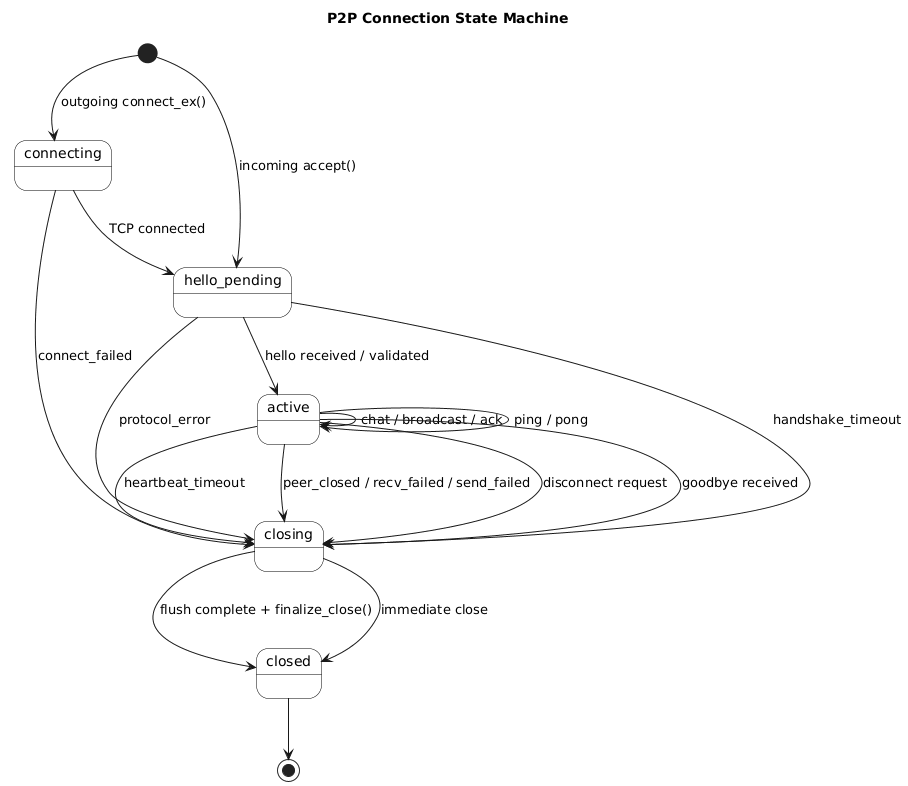
\includegraphics[width=\textwidth]{assets/diagrams/p2p-connection-state-machine.png}
\caption{State machine của một kết nối P2P trong PeerManager}
\end{figure}

\subsection{Chat và broadcast semantics}
Hai loại data message chính là \texttt{chat} và \texttt{broadcast}. Cả hai đều dùng chung một schema:
\begin{itemize}[leftmargin=2em]
    \item có \texttt{from\_peer\_id}, \texttt{to\_peer\_id}, \texttt{message\_id}, \texttt{timestamp};
    \item \texttt{payload} phải chứa \texttt{text};
    \item \texttt{ack\_required} phải là boolean.
\end{itemize}

\texttt{send\_chat()} queue đúng một message đến một peer active. Trong khi đó, \texttt{broadcast()} lặp qua tất cả peer đang \texttt{active} và queue một frame \texttt{broadcast} riêng cho từng peer.

Điểm cần nhấn mạnh là:
\begin{itemize}[leftmargin=2em]
    \item broadcast trong implementation hiện tại là fan-out trực tiếp đến các peer active;
    \item tracker không relay \texttt{broadcast};
    \item kết quả \texttt{queued\_count} chỉ có nghĩa là message đã được đưa vào outbound buffer cục bộ, chưa có nghĩa là tất cả peer đã nhận xong.
\end{itemize}

\subsection{ACK semantics}
Giao thức chạy trên TCP, nhưng vẫn dùng \texttt{ack} ở tầng ứng dụng. Lý do là TCP chỉ đảm bảo byte stream đến được đầu socket bên kia, còn hệ thống vẫn cần biết message đã:
\begin{itemize}[leftmargin=2em]
    \item được decode thành frame hoàn chỉnh;
    \item vượt qua validation;
    \item được chấp nhận ở mức runtime.
\end{itemize}

Trong implementation hiện tại:
\begin{itemize}[leftmargin=2em]
    \item khi gửi \texttt{chat} hoặc \texttt{broadcast}, sender tạo \texttt{message\_id} và ghi trạng thái ban đầu là \texttt{pending} trong \texttt{pending\_acks};
    \item khi receiver nhận message hợp lệ và thấy \texttt{ack\_required = True}, nó gọi \texttt{\_send\_ack()};
    \item khi sender nhận \texttt{ack}, trạng thái message được cập nhật thành \texttt{received}.
\end{itemize}

\texttt{ack} ở đây chỉ là \textit{delivery confirmation} ở mức runtime, không có nghĩa là:
\begin{itemize}[leftmargin=2em]
    \item guaranteed delivery;
    \item retry tự động;
    \item exactly-once delivery;
    \item persistence bền vững sau khi process chết.
\end{itemize}

Việc theo dõi ACK được lộ ra ngoài qua endpoint \texttt{/message-status}. Nếu một peer bị đóng kết nối trong lúc còn ACK pending, các bản ghi liên quan sẽ bị cập nhật thành \texttt{peer\_disconnected}.

\subsection{Heartbeat và peer liveness}
Sau khi kết nối trở thành \texttt{active}, hệ thống dùng \texttt{ping} / \texttt{pong} để kiểm tra liveness và ước lượng RTT:
\begin{itemize}[leftmargin=2em]
    \item cứ mỗi \texttt{ping\_interval}, event loop queue một \texttt{ping} kèm \texttt{ping\_id};
    \item receiver trả về \texttt{pong} với cùng \texttt{ping\_id};
    \item sender lấy thời điểm gửi trong \texttt{pending\_pings} để tính \texttt{last\_rtt\_ms}.
\end{itemize}

Nếu quá lâu không nhận được bất kỳ activity nào từ peer bên kia, \texttt{last\_seen} sẽ trở nên cũ và \texttt{\_timeout\_tick()} đóng kết nối với lý do \texttt{heartbeat\_timeout}. Vì vậy, heartbeat đóng vai trò vừa là kiểm tra sống/chết, vừa là cơ sở cleanup kết nối treo.

\subsection{Protocol errors}
Hệ thống xử lý lỗi giao thức theo hướng strict validation:
\begin{itemize}[leftmargin=2em]
    \item frame quá lớn bị lỗi \texttt{frame\_too\_large};
    \item JSON sai cú pháp bị lỗi \texttt{malformed\_json};
    \item thiếu field, sai kiểu, sai version hoặc sai schema bị báo lỗi tương ứng;
    \item message đến sai thời điểm handshake bị lỗi \texttt{handshake\_incomplete}.
\end{itemize}

Nếu còn xác định được peer gửi một cách an toàn, runtime sẽ queue một message \texttt{error} trả lại. Tuy nhiên, implementation cũng tránh tạo vòng lặp lỗi: một \texttt{error} không hợp lệ sẽ không sinh thêm \texttt{error} khác vô hạn.

\subsection{Goodbye và graceful disconnect}
Khi một peer muốn đóng kết nối chủ động, \texttt{\_initiate\_disconnect()} sẽ:
\begin{enumerate}[leftmargin=2em]
    \item chuyển trạng thái sang \texttt{closing};
    \item queue một message \texttt{goodbye} nếu kết nối vẫn còn hợp lệ;
    \item đặt cờ \texttt{close\_after\_flush = True};
    \item chờ event loop gửi hết \texttt{send\_buffer};
    \item chỉ sau đó mới \texttt{unregister} socket và chuyển sang \texttt{closed}.
\end{enumerate}

Ở phía bên kia, nếu nhận \texttt{goodbye}, runtime đóng kết nối với lý do \texttt{peer\_goodbye:<reason>}. Cơ chế này giúp hệ thống đóng socket một cách có kiểm soát, thay vì cắt kết nối đột ngột và làm mất phần dữ liệu còn đang chờ gửi.

\subsection{Kết luận}
Giao thức P2P của hệ thống là một giao thức frame-based tương đối nhỏ nhưng đầy đủ các thành phần thiết yếu:
\begin{itemize}[leftmargin=2em]
    \item framing length-prefixed trên TCP;
    \item schema validation chặt chẽ cho từng message type;
    \item state machine rõ ràng từ \texttt{connecting} đến \texttt{closed};
    \item ACK, heartbeat, protocol error và graceful disconnect ở tầng ứng dụng.
\end{itemize}

Chính giao thức này là nền tảng để các phần phía trên như direct chat, broadcast, và DHT-based channeling có thể hoạt động ổn định trên cùng một runtime transport.
